% Options for packages loaded elsewhere
\PassOptionsToPackage{unicode}{hyperref}
\PassOptionsToPackage{hyphens}{url}
%
\documentclass[
]{article}
\title{Challenge infections - Descreptive statistics}
\author{}
\date{\vspace{-2.5em}}

\usepackage{amsmath,amssymb}
\usepackage{lmodern}
\usepackage{iftex}
\ifPDFTeX
  \usepackage[T1]{fontenc}
  \usepackage[utf8]{inputenc}
  \usepackage{textcomp} % provide euro and other symbols
\else % if luatex or xetex
  \usepackage{unicode-math}
  \defaultfontfeatures{Scale=MatchLowercase}
  \defaultfontfeatures[\rmfamily]{Ligatures=TeX,Scale=1}
\fi
% Use upquote if available, for straight quotes in verbatim environments
\IfFileExists{upquote.sty}{\usepackage{upquote}}{}
\IfFileExists{microtype.sty}{% use microtype if available
  \usepackage[]{microtype}
  \UseMicrotypeSet[protrusion]{basicmath} % disable protrusion for tt fonts
}{}
\makeatletter
\@ifundefined{KOMAClassName}{% if non-KOMA class
  \IfFileExists{parskip.sty}{%
    \usepackage{parskip}
  }{% else
    \setlength{\parindent}{0pt}
    \setlength{\parskip}{6pt plus 2pt minus 1pt}}
}{% if KOMA class
  \KOMAoptions{parskip=half}}
\makeatother
\usepackage{xcolor}
\IfFileExists{xurl.sty}{\usepackage{xurl}}{} % add URL line breaks if available
\IfFileExists{bookmark.sty}{\usepackage{bookmark}}{\usepackage{hyperref}}
\hypersetup{
  pdftitle={Challenge infections - Descreptive statistics},
  hidelinks,
  pdfcreator={LaTeX via pandoc}}
\urlstyle{same} % disable monospaced font for URLs
\usepackage[margin=1in]{geometry}
\usepackage{color}
\usepackage{fancyvrb}
\newcommand{\VerbBar}{|}
\newcommand{\VERB}{\Verb[commandchars=\\\{\}]}
\DefineVerbatimEnvironment{Highlighting}{Verbatim}{commandchars=\\\{\}}
% Add ',fontsize=\small' for more characters per line
\usepackage{framed}
\definecolor{shadecolor}{RGB}{248,248,248}
\newenvironment{Shaded}{\begin{snugshade}}{\end{snugshade}}
\newcommand{\AlertTok}[1]{\textcolor[rgb]{0.94,0.16,0.16}{#1}}
\newcommand{\AnnotationTok}[1]{\textcolor[rgb]{0.56,0.35,0.01}{\textbf{\textit{#1}}}}
\newcommand{\AttributeTok}[1]{\textcolor[rgb]{0.77,0.63,0.00}{#1}}
\newcommand{\BaseNTok}[1]{\textcolor[rgb]{0.00,0.00,0.81}{#1}}
\newcommand{\BuiltInTok}[1]{#1}
\newcommand{\CharTok}[1]{\textcolor[rgb]{0.31,0.60,0.02}{#1}}
\newcommand{\CommentTok}[1]{\textcolor[rgb]{0.56,0.35,0.01}{\textit{#1}}}
\newcommand{\CommentVarTok}[1]{\textcolor[rgb]{0.56,0.35,0.01}{\textbf{\textit{#1}}}}
\newcommand{\ConstantTok}[1]{\textcolor[rgb]{0.00,0.00,0.00}{#1}}
\newcommand{\ControlFlowTok}[1]{\textcolor[rgb]{0.13,0.29,0.53}{\textbf{#1}}}
\newcommand{\DataTypeTok}[1]{\textcolor[rgb]{0.13,0.29,0.53}{#1}}
\newcommand{\DecValTok}[1]{\textcolor[rgb]{0.00,0.00,0.81}{#1}}
\newcommand{\DocumentationTok}[1]{\textcolor[rgb]{0.56,0.35,0.01}{\textbf{\textit{#1}}}}
\newcommand{\ErrorTok}[1]{\textcolor[rgb]{0.64,0.00,0.00}{\textbf{#1}}}
\newcommand{\ExtensionTok}[1]{#1}
\newcommand{\FloatTok}[1]{\textcolor[rgb]{0.00,0.00,0.81}{#1}}
\newcommand{\FunctionTok}[1]{\textcolor[rgb]{0.00,0.00,0.00}{#1}}
\newcommand{\ImportTok}[1]{#1}
\newcommand{\InformationTok}[1]{\textcolor[rgb]{0.56,0.35,0.01}{\textbf{\textit{#1}}}}
\newcommand{\KeywordTok}[1]{\textcolor[rgb]{0.13,0.29,0.53}{\textbf{#1}}}
\newcommand{\NormalTok}[1]{#1}
\newcommand{\OperatorTok}[1]{\textcolor[rgb]{0.81,0.36,0.00}{\textbf{#1}}}
\newcommand{\OtherTok}[1]{\textcolor[rgb]{0.56,0.35,0.01}{#1}}
\newcommand{\PreprocessorTok}[1]{\textcolor[rgb]{0.56,0.35,0.01}{\textit{#1}}}
\newcommand{\RegionMarkerTok}[1]{#1}
\newcommand{\SpecialCharTok}[1]{\textcolor[rgb]{0.00,0.00,0.00}{#1}}
\newcommand{\SpecialStringTok}[1]{\textcolor[rgb]{0.31,0.60,0.02}{#1}}
\newcommand{\StringTok}[1]{\textcolor[rgb]{0.31,0.60,0.02}{#1}}
\newcommand{\VariableTok}[1]{\textcolor[rgb]{0.00,0.00,0.00}{#1}}
\newcommand{\VerbatimStringTok}[1]{\textcolor[rgb]{0.31,0.60,0.02}{#1}}
\newcommand{\WarningTok}[1]{\textcolor[rgb]{0.56,0.35,0.01}{\textbf{\textit{#1}}}}
\usepackage{graphicx}
\makeatletter
\def\maxwidth{\ifdim\Gin@nat@width>\linewidth\linewidth\else\Gin@nat@width\fi}
\def\maxheight{\ifdim\Gin@nat@height>\textheight\textheight\else\Gin@nat@height\fi}
\makeatother
% Scale images if necessary, so that they will not overflow the page
% margins by default, and it is still possible to overwrite the defaults
% using explicit options in \includegraphics[width, height, ...]{}
\setkeys{Gin}{width=\maxwidth,height=\maxheight,keepaspectratio}
% Set default figure placement to htbp
\makeatletter
\def\fps@figure{htbp}
\makeatother
\setlength{\emergencystretch}{3em} % prevent overfull lines
\providecommand{\tightlist}{%
  \setlength{\itemsep}{0pt}\setlength{\parskip}{0pt}}
\setcounter{secnumdepth}{-\maxdimen} % remove section numbering
\ifLuaTeX
  \usepackage{selnolig}  % disable illegal ligatures
\fi

\begin{document}
\maketitle

\hypertarget{challenge-infections-with-eimeria.-here-i-am-presenting-some-summary-statistics-on-the-laboratory-infection-of-mice-with-different-eimeria-strains.}{%
\paragraph{\texorpdfstring{Challenge infections with \emph{Eimeria}.
Here I am presenting some summary statistics on the laboratory infection
of mice with different \emph{Eimeria}
strains.}{Challenge infections with Eimeria. Here I am presenting some summary statistics on the laboratory infection of mice with different Eimeria strains.}}\label{challenge-infections-with-eimeria.-here-i-am-presenting-some-summary-statistics-on-the-laboratory-infection-of-mice-with-different-eimeria-strains.}}

Here is a data frame containing all information derived from the
experimental infections with \emph{Eimeria}.

\begin{Shaded}
\begin{Highlighting}[]
\DocumentationTok{\#\#\#\# Read the file}
\NormalTok{CI }\OtherTok{\textless{}{-}} \FunctionTok{read.csv}\NormalTok{(}\StringTok{"https://raw.githubusercontent.com/derele/Eimeria\_Lab/master/data\_products/Challenge\_infections.csv"}\NormalTok{)}
\end{Highlighting}
\end{Shaded}

\hypertarget{wrangling}{%
\subsubsection{Wrangling}\label{wrangling}}

\begin{verbatim}
## # A tibble: 2,984 x 98
##    EH_ID experiment primary_infecti~ challenge_infec~ mouse_strain labels weight
##    <chr> <chr>      <chr>            <chr>            <chr>        <chr>   <dbl>
##  1 LM02~ E57        E88              E64              BUSNA_STRA   E57aA~   22.2
##  2 LM02~ E57        E88              E64              BUSNA_STRA   E57aB~   19.1
##  3 LM02~ E57        E88              E64              BUSNA_STRA   E57bx~   22.9
##  4 LM02~ E57        E88              E64              BUSNA_STRA   E57aP~   22  
##  5 LM02~ E57        E88              E64              BUSNA_STRA   E57aF~   20.0
##  6 LM02~ E57        E88              E64              BUSNA_STRA   E57aN~   22.1
##  7 LM02~ E57        E88              E64              BUSNA_STRA   E57bx~   22.9
##  8 LM02~ E57        E88              E64              BUSNA_STRA   E57bx~   23.2
##  9 LM02~ E57        E88              E64              BUSNA_STRA   E57bx~   23.1
## 10 LM02~ E57        E88              E64              BUSNA_STRA   E57aG~   21.0
## # ... with 2,974 more rows, and 91 more variables: weight_dpi0 <dbl>,
## #   relative_weight <dbl>, feces_weight <dbl>, dpi <int>, infection <chr>,
## #   oocyst_sq1 <int>, oocyst_sq2 <int>, oocyst_sq3 <int>, oocyst_sq4 <int>,
## #   dilution <dbl>, OO4sq <int>, OOC <dbl>, infection_history <chr>,
## #   Eim_MC <lgl>, delta <dbl>, IFNy_CEWE <dbl>, IFNy_MES <dbl>, CXCR3 <dbl>,
## #   IRG6 <dbl>, IL.12 <dbl>, CASP1 <dbl>, CXCL9 <dbl>, CXCR3_bio <dbl>,
## #   IDO1 <dbl>, IFNy <dbl>, IL.10 <dbl>, IL.12A <dbl>, IL1RN <dbl>, ...
\end{verbatim}

Let's add a column with the parasite names

\hypertarget{summary-statistics-on-experimental-design}{%
\subsubsection{Summary statistics on experimental
design}\label{summary-statistics-on-experimental-design}}

\hypertarget{summarizing-data-by-each-mouse}{%
\paragraph{Summarizing data by each
mouse}\label{summarizing-data-by-each-mouse}}

\begin{verbatim}
## Warning in max(OOC, na.rm = TRUE): no non-missing arguments to max; returning
## -Inf

## Warning in max(OOC, na.rm = TRUE): no non-missing arguments to max; returning
## -Inf

## Warning in max(OOC, na.rm = TRUE): no non-missing arguments to max; returning
## -Inf

## Warning in max(OOC, na.rm = TRUE): no non-missing arguments to max; returning
## -Inf

## Warning in max(OOC, na.rm = TRUE): no non-missing arguments to max; returning
## -Inf

## Warning in max(OOC, na.rm = TRUE): no non-missing arguments to max; returning
## -Inf

## Warning in max(OOC, na.rm = TRUE): no non-missing arguments to max; returning
## -Inf
\end{verbatim}

\begin{verbatim}
## Warning in min(relative_weight, na.rm = TRUE): no non-missing arguments to min;
## returning Inf

## Warning in min(relative_weight, na.rm = TRUE): no non-missing arguments to min;
## returning Inf

## Warning in min(relative_weight, na.rm = TRUE): no non-missing arguments to min;
## returning Inf

## Warning in min(relative_weight, na.rm = TRUE): no non-missing arguments to min;
## returning Inf

## Warning in min(relative_weight, na.rm = TRUE): no non-missing arguments to min;
## returning Inf

## Warning in min(relative_weight, na.rm = TRUE): no non-missing arguments to min;
## returning Inf
\end{verbatim}

\begin{verbatim}
## `summarise()` has grouped output by 'EH_ID'. You can override using the `.groups` argument.
\end{verbatim}

\hypertarget{how-many-mice-do-we-have-in-each-infection-primary-or-challenge-infection}{%
\paragraph{How many mice do we have in each infection ? (primary or
challenge
infection)}\label{how-many-mice-do-we-have-in-each-infection-primary-or-challenge-infection}}

\begin{verbatim}
## # A tibble: 2 x 2
##   infection total_mice
##   <chr>          <int>
## 1 challenge        132
## 2 primary          153
\end{verbatim}

\hypertarget{how-many-experiments-do-we-have-how-many-mice-are-in-each-experiment}{%
\paragraph{How many experiments do we have? How many mice are in each
experiment?}\label{how-many-experiments-do-we-have-how-many-mice-are-in-each-experiment}}

\begin{verbatim}
## # A tibble: 5 x 2
##   experiment total_mice
##   <chr>           <int>
## 1 E10                52
## 2 E11                55
## 3 E57               106
## 4 P3                 32
## 5 P4                 40
\end{verbatim}

\hypertarget{how-many-mouse-strains-do-we-have}{%
\paragraph{How many mouse strains do we
have?}\label{how-many-mouse-strains-do-we-have}}

We here use four wild-derived inbred mouse strains. from these mouse
strains F1 hybrids were generated.

Two parental strains represented M. m. domesticus: - SCHUNT (Locality:
Schweben, Hessen, Germany {[}N: 5°0 26′, E: 9°36′{]} (Martincová et al.,
2019))\\
- STRA (Locality: Straas, Bavaria, Germany {[}N: 50°11′, E: 11°46′{]}
(Piálek et al., 2008), Two parental strains represented M. m. musculus:
- BUSNA (Locality: Buškovice, Bohemia, Czech Republic {[}N: 5°0 14′, E:
1°3 22′{]} (Piálek et al., 2008)) - PWD (Locality: Kunratice, Bohemia,
Czech Republic {[}N: 5°0 01′, E: 14 2°9′{]} (Gregorová \& Forejt, 2000))

\begin{verbatim}
## `summarise()` has grouped output by 'mouse_strain'. You can override using the `.groups` argument.
\end{verbatim}

\begin{verbatim}
## # A tibble: 13 x 3
## # Groups:   mouse_strain [13]
##    mouse_strain  hybrid_status       total_mice
##    <chr>         <chr>                    <int>
##  1 BUSNA_BUSNA   F0 M. m. musculus            8
##  2 BUSNA_PWD     F1 M. m. musculus            6
##  3 BUSNA_STRA    F1 hybrid                   10
##  4 NMRI          other                       72
##  5 PWD_BUSNA     F1 M. m. musculus            8
##  6 PWD_PWD       F0 M. m. musculus           56
##  7 PWD_SCHUNT    F1 hybrid                    6
##  8 SCHUNT_PWD    F1 hybrid                    8
##  9 SCHUNT_SCHUNT F0 M. m. domesticus         73
## 10 SCHUNT_STRA   F1 M. m. domesticus          6
## 11 STRA_BUSNA    F1 hybrid                   10
## 12 STRA_SCHUNT   F1 M. m. domesticus         10
## 13 STRA_STRA     F0 M. m. domesticus         12
\end{verbatim}

\begin{verbatim}
## # A tibble: 6 x 2
##   hybrid_status       total_mice
##   <chr>                    <int>
## 1 F0 M. m. domesticus         85
## 2 F0 M. m. musculus           64
## 3 F1 hybrid                   34
## 4 F1 M. m. domesticus         16
## 5 F1 M. m. musculus           14
## 6 other                       72
\end{verbatim}

\hypertarget{which-eimeria-strains-were-used}{%
\paragraph{Which Eimeria strains were
used?}\label{which-eimeria-strains-were-used}}

The three parasite isolates used in this study were isolated from feces
of three different M. m. domesticus/M. m. musculus hybrid mice captured
in Brandenburg, Germany, in 2016 (capture permit No.~2347/35/2014). The
parasite isolates belong to both the most prevalent Eimeria species in
this area, namely E. ferrisi (isolate Brandenburg64) and E. falciformis
(isolate Brandenburg88)(Jarquín-Díaz et al., 2019). Isolate
Brandenburg64 was isolated in a 92\% M. m. domesticus individual (hybrid
index (HI) = 0.08: Proportion of M. m. musculus alleles in a set of 14
diagnostic markers, see Balard et al.~(2020)) and isolate Brandenburg88
in a 80\% M. m. domesticus (HI = 0.2).

Prepatency and the peak day of parasite shedding for these isolates were
estimated during infection in NMRI laboratory mice (Al-khlifeh et al.,
2019) which were also used for serial passaging of the isolates.
Previous to the experiment, the isolates had been passaged,
respectively, 3 and 4 times in NMRI laboratory mice. Parasite infective
forms (oocysts) were recovered by flotation in saturated NaCl solution
followed by washing and observation under light microscope (following
the protocol described in Clerc et al.~(2019)) and stored at room
temperature in 1 ml of 2\% potassium dichromate for a maximum of 2
months before infection of the wild-derived mice. Oocysts were allowed
to sporulate 10 days before infection in a water bath at 30°C

\begin{enumerate}
\def\labelenumi{\arabic{enumi}.}
\tightlist
\item
  Primary:
\end{enumerate}

\begin{verbatim}
## # A tibble: 3 x 2
##   Parasite_primary    total_mice
##   <chr>                    <int>
## 1 Eimeria falciformis         60
## 2 Eimeria ferrisi             69
## 3 uninfected                  24
\end{verbatim}

\begin{enumerate}
\def\labelenumi{\arabic{enumi}.}
\setcounter{enumi}{1}
\tightlist
\item
  Further, for the challenge infections
\end{enumerate}

\begin{verbatim}
## # A tibble: 3 x 2
##   Parasite_challenge  total_mice
##   <chr>                    <int>
## 1 Eimeria falciformis         27
## 2 Eimeria ferrisi             54
## 3 uninfected                  51
\end{verbatim}

\hypertarget{how-many-mice-died-in-each-infection}{%
\paragraph{2.6 How many mice died in each
infection?}\label{how-many-mice-died-in-each-infection}}

\begin{verbatim}
## # A tibble: 2 x 2
##   death     `length(EH_ID)`
##   <chr>               <int>
## 1 challenge             264
## 2 primary                21
\end{verbatim}

\hypertarget{from-the-mice-that-died-in-the-primary-infection-what-was-the-infection-status}{%
\paragraph{2.6.1 From the mice that died in the primary infection, what
was the infection
status?}\label{from-the-mice-that-died-in-the-primary-infection-what-was-the-infection-status}}

\begin{verbatim}
## # A tibble: 2 x 2
##   Parasite_primary    total_mice
##   <chr>                    <int>
## 1 Eimeria falciformis         18
## 2 Eimeria ferrisi              3
\end{verbatim}

Most of the mice dying in the first infections are infected with Eimeria
falciformis.

\hypertarget{summary-statistics---resistance-tolerance-proxies}{%
\subsubsection{3 Summary statistics - Resistance/ Tolerance
proxies}\label{summary-statistics---resistance-tolerance-proxies}}

\hypertarget{what-is-the-avarege-maximum-oocysts-output-for-each-mouse-in-the-primary-and-challenge-infections}{%
\paragraph{3.1 What is the avarege maximum oocysts output for each mouse
in the primary and challenge
infections?}\label{what-is-the-avarege-maximum-oocysts-output-for-each-mouse-in-the-primary-and-challenge-infections}}

\begin{enumerate}
\def\labelenumi{\arabic{enumi}.}
\tightlist
\item
  Visualizing the primary infections `
\end{enumerate}

\begin{Shaded}
\begin{Highlighting}[]
\NormalTok{CIMouse }\SpecialCharTok{\%\textgreater{}\%}
    \FunctionTok{filter}\NormalTok{(infection }\SpecialCharTok{==} \StringTok{"primary"}\NormalTok{)  }\SpecialCharTok{\%\textgreater{}\%}
  \FunctionTok{ggplot}\NormalTok{(}\FunctionTok{aes}\NormalTok{(max\_OOC, }\AttributeTok{color =}\NormalTok{ Parasite\_primary, }\AttributeTok{fill =}\NormalTok{ Parasite\_primary)) }\SpecialCharTok{+}
  \FunctionTok{geom\_histogram}\NormalTok{(}\AttributeTok{bins =} \DecValTok{30}\NormalTok{, }\AttributeTok{alpha =} \FloatTok{0.5}\NormalTok{) }\SpecialCharTok{+}
  \FunctionTok{labs}\NormalTok{(}\AttributeTok{x =} \StringTok{"Oocysts at day of maximal shedding"}\NormalTok{, }\AttributeTok{y =} \StringTok{"Number of mice"}\NormalTok{,}
       \AttributeTok{title =} \StringTok{"Maximum oocyst shedding per mouse, primary infections"}\NormalTok{) }\SpecialCharTok{+}
    \FunctionTok{theme\_bw}\NormalTok{()}
\end{Highlighting}
\end{Shaded}

\includegraphics{Descriptive_stats_files/figure-latex/unnamed-chunk-13-1.pdf}

\begin{Shaded}
\begin{Highlighting}[]
\NormalTok{CIMouse  }\SpecialCharTok{\%\textgreater{}\%}
    \FunctionTok{filter}\NormalTok{(infection }\SpecialCharTok{==} \StringTok{"primary"}\NormalTok{)  }\SpecialCharTok{\%\textgreater{}\%}
  \FunctionTok{ggplot}\NormalTok{(}\FunctionTok{aes}\NormalTok{(}\AttributeTok{x =}\NormalTok{ Parasite\_primary, }\AttributeTok{y =}\NormalTok{ max\_OOC, }\AttributeTok{fill =}\NormalTok{ Parasite\_primary)) }\SpecialCharTok{+}
  \FunctionTok{geom\_boxplot}\NormalTok{() }\SpecialCharTok{+}
    \FunctionTok{theme\_bw}\NormalTok{()}
\end{Highlighting}
\end{Shaded}

\includegraphics{Descriptive_stats_files/figure-latex/unnamed-chunk-13-2.pdf}

\begin{Shaded}
\begin{Highlighting}[]
\NormalTok{CIMouse  }\SpecialCharTok{\%\textgreater{}\%}
    \FunctionTok{filter}\NormalTok{(infection }\SpecialCharTok{==} \StringTok{"primary"}\NormalTok{)  }\SpecialCharTok{\%\textgreater{}\%}
  \FunctionTok{ggplot}\NormalTok{(}\FunctionTok{aes}\NormalTok{(}\AttributeTok{x =}\NormalTok{ Parasite\_primary, }\AttributeTok{y =}\NormalTok{ max\_OOC, }\AttributeTok{fill =}\NormalTok{ Parasite\_primary)) }\SpecialCharTok{+}
  \FunctionTok{geom\_violin}\NormalTok{() }\SpecialCharTok{+}
    \FunctionTok{theme\_bw}\NormalTok{() }
\end{Highlighting}
\end{Shaded}

\includegraphics{Descriptive_stats_files/figure-latex/unnamed-chunk-13-3.pdf}

\begin{Shaded}
\begin{Highlighting}[]
\NormalTok{CIMouse  }\SpecialCharTok{\%\textgreater{}\%}
    \FunctionTok{filter}\NormalTok{(infection }\SpecialCharTok{==} \StringTok{"primary"}\NormalTok{, }\SpecialCharTok{!}\NormalTok{Parasite\_primary }\SpecialCharTok{==} \StringTok{"uninfected"}\NormalTok{)  }\SpecialCharTok{\%\textgreater{}\%}
  \FunctionTok{ggplot}\NormalTok{(}\FunctionTok{aes}\NormalTok{(}\AttributeTok{x =}\NormalTok{ Parasite\_primary, }\AttributeTok{y =}\NormalTok{ max\_OOC, }\AttributeTok{fill =}\NormalTok{ Parasite\_primary)) }\SpecialCharTok{+}
  \FunctionTok{geom\_violin}\NormalTok{(}\AttributeTok{alpha =} \FloatTok{0.5}\NormalTok{) }\SpecialCharTok{+}
    \FunctionTok{geom\_line}\NormalTok{() }\SpecialCharTok{+}
     \FunctionTok{stat\_summary}\NormalTok{(}\AttributeTok{fun.y =} \StringTok{"median"}\NormalTok{, }\AttributeTok{geom =} \StringTok{"point"}\NormalTok{, }\AttributeTok{size =} \DecValTok{3}\NormalTok{) }\SpecialCharTok{+}
    \FunctionTok{theme\_bw}\NormalTok{() }
\end{Highlighting}
\end{Shaded}

\begin{verbatim}
## Warning: `fun.y` is deprecated. Use `fun` instead.
\end{verbatim}

\includegraphics{Descriptive_stats_files/figure-latex/unnamed-chunk-13-4.pdf}

\begin{Shaded}
\begin{Highlighting}[]
\NormalTok{CIMouse  }\SpecialCharTok{\%\textgreater{}\%}
    \FunctionTok{filter}\NormalTok{(infection }\SpecialCharTok{==} \StringTok{"primary"}\NormalTok{, }\SpecialCharTok{!}\NormalTok{Parasite\_primary }\SpecialCharTok{==} \StringTok{"uninfected"}\NormalTok{)  }\SpecialCharTok{\%\textgreater{}\%}
  \FunctionTok{ggplot}\NormalTok{(}\FunctionTok{aes}\NormalTok{(}\AttributeTok{x =}\NormalTok{ Parasite\_primary, }\AttributeTok{y =}\NormalTok{ max\_OOC, }\AttributeTok{fill =}\NormalTok{ Parasite\_primary)) }\SpecialCharTok{+}
  \FunctionTok{geom\_violin}\NormalTok{(}\AttributeTok{alpha =} \FloatTok{0.5}\NormalTok{) }\SpecialCharTok{+}
    \FunctionTok{geom\_line}\NormalTok{() }\SpecialCharTok{+}
     \FunctionTok{stat\_summary}\NormalTok{(}\AttributeTok{fun.y =} \StringTok{"median"}\NormalTok{, }\AttributeTok{geom =} \StringTok{"point"}\NormalTok{, }\AttributeTok{size =} \DecValTok{3}\NormalTok{) }\SpecialCharTok{+}
    \FunctionTok{theme\_bw}\NormalTok{() }
\end{Highlighting}
\end{Shaded}

\begin{verbatim}
## Warning: `fun.y` is deprecated. Use `fun` instead.
\end{verbatim}

\includegraphics{Descriptive_stats_files/figure-latex/unnamed-chunk-13-5.pdf}

\begin{enumerate}
\def\labelenumi{\arabic{enumi}.}
\setcounter{enumi}{1}
\tightlist
\item
  And the challenge infections
\end{enumerate}

\begin{Shaded}
\begin{Highlighting}[]
\NormalTok{CIMouse }\SpecialCharTok{\%\textgreater{}\%}
    \FunctionTok{filter}\NormalTok{(infection }\SpecialCharTok{==} \StringTok{"challenge"}\NormalTok{)  }\SpecialCharTok{\%\textgreater{}\%}
  \FunctionTok{ggplot}\NormalTok{(}\FunctionTok{aes}\NormalTok{(max\_OOC, }\AttributeTok{color =}\NormalTok{ Parasite\_challenge, }\AttributeTok{fill =}\NormalTok{ Parasite\_challenge)) }\SpecialCharTok{+}
  \FunctionTok{geom\_histogram}\NormalTok{(}\AttributeTok{bins =} \DecValTok{30}\NormalTok{, }\AttributeTok{alpha =} \FloatTok{0.5}\NormalTok{) }\SpecialCharTok{+}
  \FunctionTok{labs}\NormalTok{(}\AttributeTok{x =} \StringTok{"Oocysts at day of maximal shedding"}\NormalTok{, }\AttributeTok{y =} \StringTok{"Number of mice"}\NormalTok{,}
       \AttributeTok{title =} \StringTok{"Maximum oocyst shedding per mouse, challenge infections"}\NormalTok{) }\SpecialCharTok{+}
    \FunctionTok{theme\_bw}\NormalTok{()}
\end{Highlighting}
\end{Shaded}

\begin{verbatim}
## Warning: Removed 7 rows containing non-finite values (stat_bin).
\end{verbatim}

\includegraphics{Descriptive_stats_files/figure-latex/unnamed-chunk-14-1.pdf}

\begin{Shaded}
\begin{Highlighting}[]
\NormalTok{CIMouse  }\SpecialCharTok{\%\textgreater{}\%}
    \FunctionTok{filter}\NormalTok{(infection }\SpecialCharTok{==} \StringTok{"challenge"}\NormalTok{)  }\SpecialCharTok{\%\textgreater{}\%}
  \FunctionTok{ggplot}\NormalTok{(}\FunctionTok{aes}\NormalTok{(}\AttributeTok{x =}\NormalTok{ Parasite\_challenge, }\AttributeTok{y =}\NormalTok{ max\_OOC, }\AttributeTok{fill =}\NormalTok{ Parasite\_challenge)) }\SpecialCharTok{+}
  \FunctionTok{geom\_boxplot}\NormalTok{() }\SpecialCharTok{+}
    \FunctionTok{theme\_bw}\NormalTok{()}
\end{Highlighting}
\end{Shaded}

\begin{verbatim}
## Warning: Removed 7 rows containing non-finite values (stat_boxplot).
\end{verbatim}

\includegraphics{Descriptive_stats_files/figure-latex/unnamed-chunk-14-2.pdf}

\begin{Shaded}
\begin{Highlighting}[]
\NormalTok{CIMouse  }\SpecialCharTok{\%\textgreater{}\%}
    \FunctionTok{filter}\NormalTok{(infection }\SpecialCharTok{==} \StringTok{"challenge"}\NormalTok{)  }\SpecialCharTok{\%\textgreater{}\%}
  \FunctionTok{ggplot}\NormalTok{(}\FunctionTok{aes}\NormalTok{(}\AttributeTok{x =}\NormalTok{ Parasite\_challenge, }\AttributeTok{y =}\NormalTok{ max\_OOC, }\AttributeTok{fill =}\NormalTok{ Parasite\_challenge)) }\SpecialCharTok{+}
  \FunctionTok{geom\_violin}\NormalTok{() }\SpecialCharTok{+}
    \FunctionTok{theme\_bw}\NormalTok{() }
\end{Highlighting}
\end{Shaded}

\begin{verbatim}
## Warning: Removed 7 rows containing non-finite values (stat_ydensity).
\end{verbatim}

\includegraphics{Descriptive_stats_files/figure-latex/unnamed-chunk-14-3.pdf}

\begin{Shaded}
\begin{Highlighting}[]
\NormalTok{CIMouse  }\SpecialCharTok{\%\textgreater{}\%}
    \FunctionTok{filter}\NormalTok{(infection }\SpecialCharTok{==} \StringTok{"challenge"}\NormalTok{, }\SpecialCharTok{!}\NormalTok{Parasite\_challenge }\SpecialCharTok{==} \StringTok{"uninfected"}\NormalTok{)  }\SpecialCharTok{\%\textgreater{}\%}
  \FunctionTok{ggplot}\NormalTok{(}\FunctionTok{aes}\NormalTok{(}\AttributeTok{x =}\NormalTok{ Parasite\_challenge, }\AttributeTok{y =}\NormalTok{ max\_OOC, }\AttributeTok{fill =}\NormalTok{ Parasite\_challenge)) }\SpecialCharTok{+}
  \FunctionTok{geom\_violin}\NormalTok{(}\AttributeTok{alpha =} \FloatTok{0.5}\NormalTok{) }\SpecialCharTok{+}
    \FunctionTok{geom\_line}\NormalTok{() }\SpecialCharTok{+}
     \FunctionTok{stat\_summary}\NormalTok{(}\AttributeTok{fun.y =} \StringTok{"median"}\NormalTok{, }\AttributeTok{geom =} \StringTok{"point"}\NormalTok{, }\AttributeTok{size =} \DecValTok{3}\NormalTok{) }\SpecialCharTok{+}
    \FunctionTok{theme\_bw}\NormalTok{() }
\end{Highlighting}
\end{Shaded}

\begin{verbatim}
## Warning: `fun.y` is deprecated. Use `fun` instead.
\end{verbatim}

\begin{verbatim}
## Warning: Removed 6 rows containing non-finite values (stat_ydensity).
\end{verbatim}

\begin{verbatim}
## Warning: Removed 6 rows containing non-finite values (stat_summary).
\end{verbatim}

\includegraphics{Descriptive_stats_files/figure-latex/unnamed-chunk-14-4.pdf}

\hypertarget{maximum-oocysts-output-for-each-mouse-strain-in-each-infection}{%
\paragraph{maximum oocysts output for each mouse strain in each
infection?}\label{maximum-oocysts-output-for-each-mouse-strain-in-each-infection}}

\begin{enumerate}
\def\labelenumi{\arabic{enumi}.}
\item
  primary infections:
  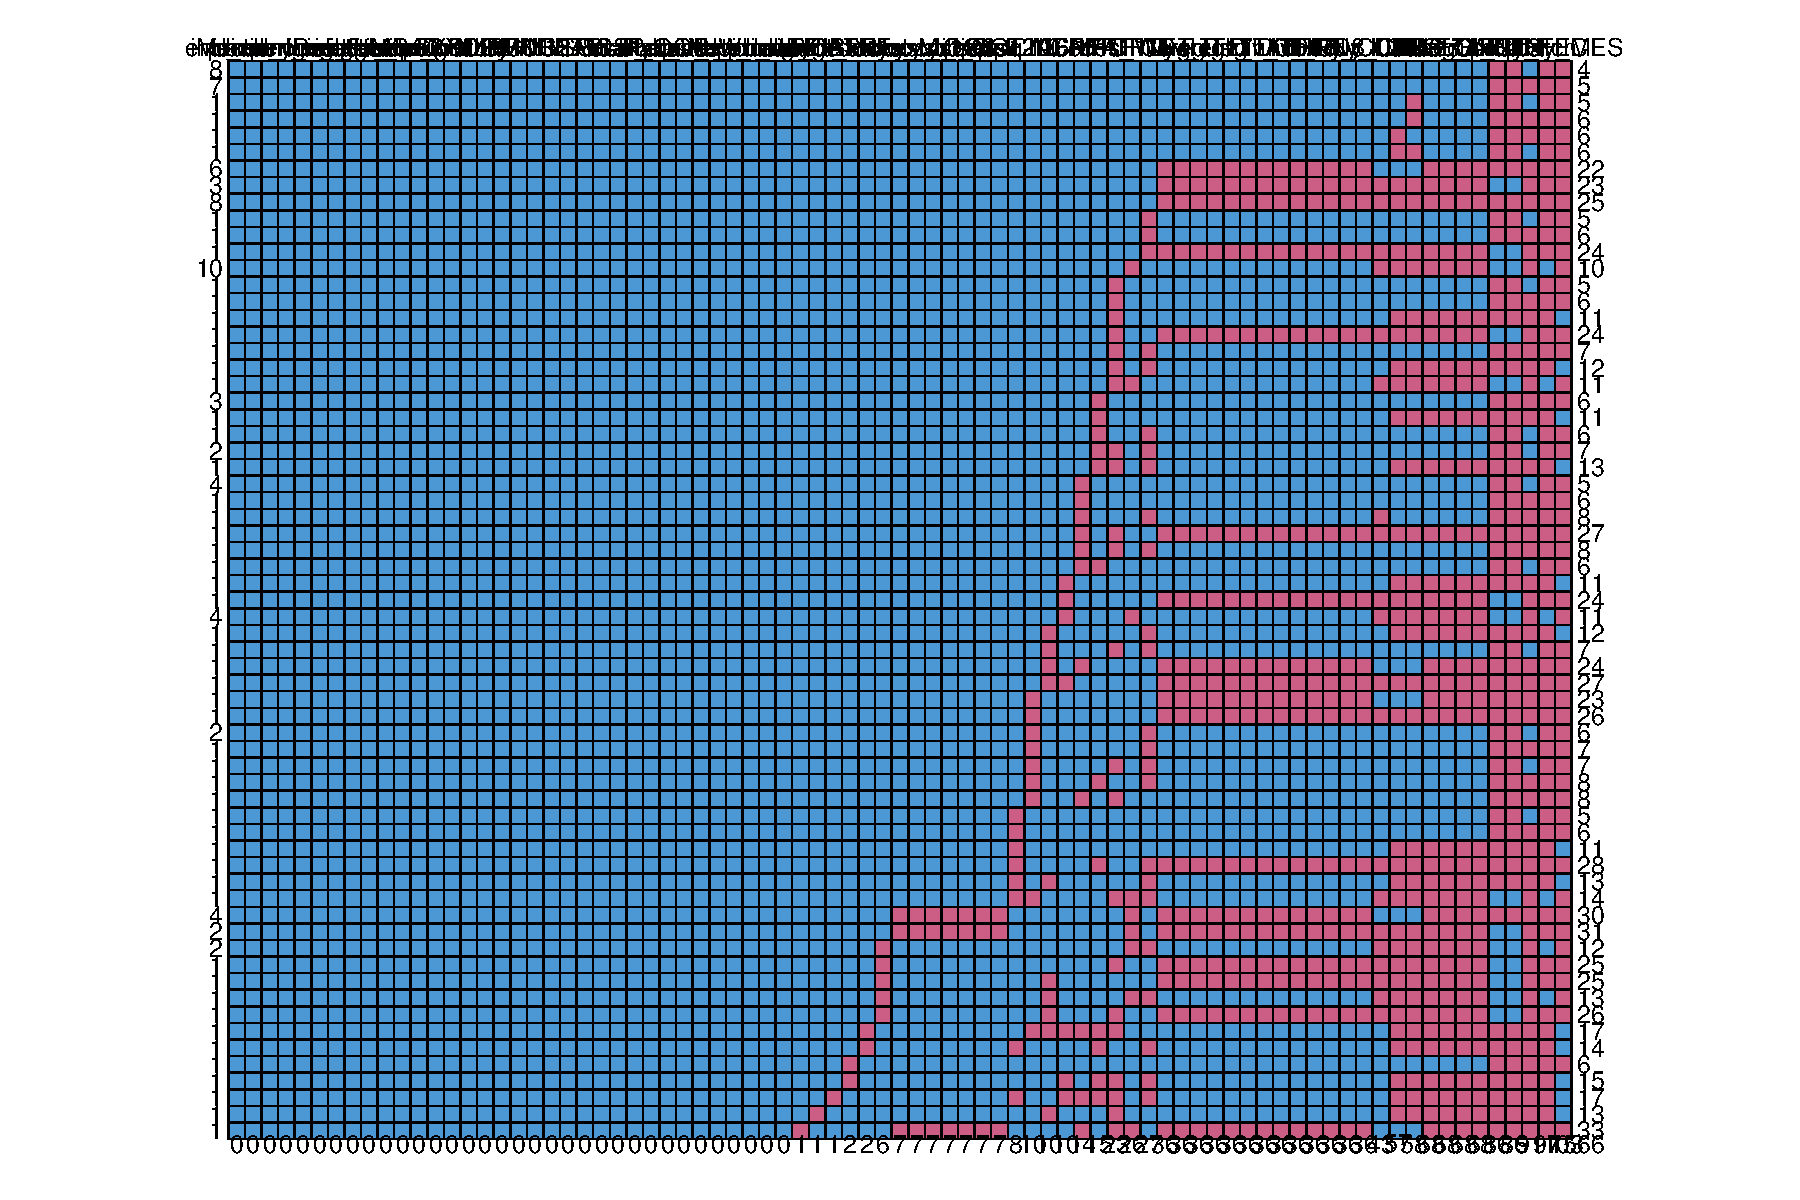
\includegraphics{Descriptive_stats_files/figure-latex/unnamed-chunk-15-1.pdf}
\item
  Challenge infections:
\end{enumerate}

\begin{verbatim}
## Warning: Removed 7 rows containing non-finite values (stat_boxplot).
\end{verbatim}

\includegraphics{Descriptive_stats_files/figure-latex/unnamed-chunk-16-1.pdf}
Effect of experiments on oocyst shedding?

\begin{enumerate}
\def\labelenumi{\arabic{enumi}.}
\item
  primary infections:
  \includegraphics{Descriptive_stats_files/figure-latex/unnamed-chunk-17-1.pdf}
\item
  Challenge infections:
\end{enumerate}

\begin{verbatim}
## Warning: Removed 7 rows containing non-finite values (stat_boxplot).
\end{verbatim}

\includegraphics{Descriptive_stats_files/figure-latex/unnamed-chunk-18-1.pdf}
Patency in primary infections

\begin{Shaded}
\begin{Highlighting}[]
\NormalTok{CI }\SpecialCharTok{\%\textgreater{}\%}
  \FunctionTok{group\_by}\NormalTok{(}\StringTok{"EH\_ID"}\NormalTok{) }\SpecialCharTok{\%\textgreater{}\%}
  \FunctionTok{filter}\NormalTok{(infection }\SpecialCharTok{==} \StringTok{"primary"}\NormalTok{) }\SpecialCharTok{\%\textgreater{}\%}
  \FunctionTok{ggplot}\NormalTok{(}\FunctionTok{aes}\NormalTok{(}\AttributeTok{x =}\NormalTok{ dpi, }\AttributeTok{y =}\NormalTok{ OOC, }\AttributeTok{color =}\NormalTok{ Parasite\_primary)) }\SpecialCharTok{+}
  \FunctionTok{geom\_point}\NormalTok{(}\AttributeTok{position =} \FunctionTok{position\_jitterdodge}\NormalTok{()) }\SpecialCharTok{+}
  \FunctionTok{labs}\NormalTok{(}\AttributeTok{x =} \StringTok{"Days Post Infection"}\NormalTok{, }\AttributeTok{y =} \StringTok{"Oocysts per gram"}\NormalTok{,}
       \AttributeTok{title =} \StringTok{"Oocyst shedding in primary infections during the }
\StringTok{       course of infection"}\NormalTok{) }\SpecialCharTok{+}
    \FunctionTok{theme\_bw}\NormalTok{() }
\end{Highlighting}
\end{Shaded}

\begin{verbatim}
## Warning: Removed 497 rows containing missing values (geom_point).
\end{verbatim}

\includegraphics{Descriptive_stats_files/figure-latex/unnamed-chunk-19-1.pdf}

Patency in primary infections - experiments

\begin{Shaded}
\begin{Highlighting}[]
\NormalTok{CI }\SpecialCharTok{\%\textgreater{}\%}
  \FunctionTok{group\_by}\NormalTok{(}\StringTok{"EH\_ID"}\NormalTok{) }\SpecialCharTok{\%\textgreater{}\%}
  \FunctionTok{filter}\NormalTok{(infection }\SpecialCharTok{==} \StringTok{"primary"}\NormalTok{) }\SpecialCharTok{\%\textgreater{}\%}
  \FunctionTok{ggplot}\NormalTok{(}\FunctionTok{aes}\NormalTok{(}\AttributeTok{x =}\NormalTok{ dpi, }\AttributeTok{y =}\NormalTok{ OOC, }\AttributeTok{color =}\NormalTok{ Parasite\_primary)) }\SpecialCharTok{+}
  \FunctionTok{geom\_point}\NormalTok{(}\AttributeTok{position =} \FunctionTok{position\_jitterdodge}\NormalTok{()) }\SpecialCharTok{+}
  \FunctionTok{labs}\NormalTok{(}\AttributeTok{x =} \StringTok{"Days Post Infection"}\NormalTok{, }\AttributeTok{y =} \StringTok{"Oocysts per gram"}\NormalTok{,}
       \AttributeTok{title =} \StringTok{"Oocyst shedding in primary infections during the }
\StringTok{       course of infection"}\NormalTok{) }\SpecialCharTok{+}
    \FunctionTok{theme\_bw}\NormalTok{() }\SpecialCharTok{+}
    \FunctionTok{facet\_wrap}\NormalTok{(}\SpecialCharTok{\textasciitilde{}}\NormalTok{ experiment)}
\end{Highlighting}
\end{Shaded}

\begin{verbatim}
## Warning: Removed 497 rows containing missing values (geom_point).
\end{verbatim}

\includegraphics{Descriptive_stats_files/figure-latex/unnamed-chunk-20-1.pdf}
Patency in primary infections - mouse strains

\begin{Shaded}
\begin{Highlighting}[]
\NormalTok{CI }\SpecialCharTok{\%\textgreater{}\%}
  \FunctionTok{group\_by}\NormalTok{(}\StringTok{"EH\_ID"}\NormalTok{) }\SpecialCharTok{\%\textgreater{}\%}
  \FunctionTok{filter}\NormalTok{(infection }\SpecialCharTok{==} \StringTok{"primary"}\NormalTok{) }\SpecialCharTok{\%\textgreater{}\%}
  \FunctionTok{ggplot}\NormalTok{(}\FunctionTok{aes}\NormalTok{(}\AttributeTok{x =}\NormalTok{ dpi, }\AttributeTok{y =}\NormalTok{ OOC, }\AttributeTok{color =}\NormalTok{ Parasite\_primary)) }\SpecialCharTok{+}
  \FunctionTok{geom\_point}\NormalTok{(}\AttributeTok{position =} \FunctionTok{position\_jitterdodge}\NormalTok{()) }\SpecialCharTok{+}
  \FunctionTok{labs}\NormalTok{(}\AttributeTok{x =} \StringTok{"Days Post Infection"}\NormalTok{, }\AttributeTok{y =} \StringTok{"Oocysts per gram"}\NormalTok{,}
       \AttributeTok{title =} \StringTok{"Oocyst shedding in primary infections during the }
\StringTok{       course of infection"}\NormalTok{) }\SpecialCharTok{+}
    \FunctionTok{theme\_bw}\NormalTok{() }\SpecialCharTok{+}
    \FunctionTok{facet\_wrap}\NormalTok{(}\SpecialCharTok{\textasciitilde{}}\NormalTok{ hybrid\_status)}
\end{Highlighting}
\end{Shaded}

\begin{verbatim}
## Warning: Removed 497 rows containing missing values (geom_point).
\end{verbatim}

\includegraphics{Descriptive_stats_files/figure-latex/unnamed-chunk-21-1.pdf}
Patency in challenge infections - experiments

\begin{Shaded}
\begin{Highlighting}[]
\NormalTok{CI }\SpecialCharTok{\%\textgreater{}\%}
  \FunctionTok{group\_by}\NormalTok{(}\StringTok{"EH\_ID"}\NormalTok{) }\SpecialCharTok{\%\textgreater{}\%}
  \FunctionTok{filter}\NormalTok{(infection }\SpecialCharTok{==} \StringTok{"challenge"}\NormalTok{) }\SpecialCharTok{\%\textgreater{}\%}
  \FunctionTok{ggplot}\NormalTok{(}\FunctionTok{aes}\NormalTok{(}\AttributeTok{x =}\NormalTok{ dpi, }\AttributeTok{y =}\NormalTok{ OOC, }\AttributeTok{color =}\NormalTok{ Parasite\_challenge)) }\SpecialCharTok{+}
  \FunctionTok{geom\_point}\NormalTok{(}\AttributeTok{position =} \FunctionTok{position\_jitterdodge}\NormalTok{()) }\SpecialCharTok{+}
  \FunctionTok{labs}\NormalTok{(}\AttributeTok{x =} \StringTok{"Days Post Infection"}\NormalTok{, }\AttributeTok{y =} \StringTok{"Oocysts per gram"}\NormalTok{,}
       \AttributeTok{title =} \StringTok{"Oocyst shedding in challenge infections during the }
\StringTok{       course of infection"}\NormalTok{) }\SpecialCharTok{+}
    \FunctionTok{theme\_bw}\NormalTok{() }\SpecialCharTok{+}
    \FunctionTok{facet\_wrap}\NormalTok{(}\SpecialCharTok{\textasciitilde{}}\NormalTok{ experiment)}
\end{Highlighting}
\end{Shaded}

\begin{verbatim}
## Warning: Removed 167 rows containing missing values (geom_point).
\end{verbatim}

\includegraphics{Descriptive_stats_files/figure-latex/unnamed-chunk-22-1.pdf}
Patency in challenge infections - mouse strains

\begin{Shaded}
\begin{Highlighting}[]
\NormalTok{CI }\SpecialCharTok{\%\textgreater{}\%}
  \FunctionTok{group\_by}\NormalTok{(}\StringTok{"EH\_ID"}\NormalTok{) }\SpecialCharTok{\%\textgreater{}\%}
  \FunctionTok{filter}\NormalTok{(infection }\SpecialCharTok{==} \StringTok{"challenge"}\NormalTok{) }\SpecialCharTok{\%\textgreater{}\%}
  \FunctionTok{ggplot}\NormalTok{(}\FunctionTok{aes}\NormalTok{(}\AttributeTok{x =}\NormalTok{ dpi, }\AttributeTok{y =}\NormalTok{ OOC, }\AttributeTok{color =}\NormalTok{ Parasite\_challenge)) }\SpecialCharTok{+}
  \FunctionTok{geom\_point}\NormalTok{(}\AttributeTok{position =} \FunctionTok{position\_jitterdodge}\NormalTok{()) }\SpecialCharTok{+}
  \FunctionTok{labs}\NormalTok{(}\AttributeTok{x =} \StringTok{"Days Post Infection"}\NormalTok{, }\AttributeTok{y =} \StringTok{"Oocysts per gram"}\NormalTok{,}
       \AttributeTok{title =} \StringTok{"Oocyst shedding in challenge infections during the }
\StringTok{       course of infection"}\NormalTok{) }\SpecialCharTok{+}
    \FunctionTok{theme\_bw}\NormalTok{() }\SpecialCharTok{+}
    \FunctionTok{facet\_wrap}\NormalTok{(}\SpecialCharTok{\textasciitilde{}}\NormalTok{ hybrid\_status)}
\end{Highlighting}
\end{Shaded}

\begin{verbatim}
## Warning: Removed 167 rows containing missing values (geom_point).
\end{verbatim}

\includegraphics{Descriptive_stats_files/figure-latex/unnamed-chunk-23-1.pdf}

\hypertarget{what-is-the-average-max-weight-loss-output-for-each-mouse-in-the-primary-and-challenge-infections}{%
\paragraph{What is the average max weight loss output for each mouse in
the primary and challenge
infections?}\label{what-is-the-average-max-weight-loss-output-for-each-mouse-in-the-primary-and-challenge-infections}}

\begin{enumerate}
\def\labelenumi{\arabic{enumi}.}
\tightlist
\item
  Visualizing the primary infections `
\end{enumerate}

\begin{Shaded}
\begin{Highlighting}[]
\NormalTok{CIMouse }\SpecialCharTok{\%\textgreater{}\%}
\NormalTok{    dplyr}\SpecialCharTok{::}\FunctionTok{filter}\NormalTok{(infection }\SpecialCharTok{==} \StringTok{"primary"}\NormalTok{) }\SpecialCharTok{\%\textgreater{}\%}
  \FunctionTok{ggplot}\NormalTok{(}\FunctionTok{aes}\NormalTok{(max\_WL, }\AttributeTok{color =}\NormalTok{ Parasite\_primary, }\AttributeTok{fill =}\NormalTok{ Parasite\_primary)) }\SpecialCharTok{+}
  \FunctionTok{geom\_histogram}\NormalTok{(}\AttributeTok{bins =} \DecValTok{30}\NormalTok{, }\AttributeTok{alpha =} \FloatTok{0.5}\NormalTok{)  }\SpecialCharTok{+}
    \FunctionTok{theme\_bw}\NormalTok{()}
\end{Highlighting}
\end{Shaded}

\includegraphics{Descriptive_stats_files/figure-latex/unnamed-chunk-24-1.pdf}

\begin{Shaded}
\begin{Highlighting}[]
\NormalTok{CIMouse  }\SpecialCharTok{\%\textgreater{}\%}
    \FunctionTok{filter}\NormalTok{(infection }\SpecialCharTok{==} \StringTok{"primary"}\NormalTok{)  }\SpecialCharTok{\%\textgreater{}\%}
  \FunctionTok{ggplot}\NormalTok{(}\FunctionTok{aes}\NormalTok{(}\AttributeTok{x =}\NormalTok{ Parasite\_primary, }\AttributeTok{y =}\NormalTok{ max\_WL, }\AttributeTok{fill =}\NormalTok{ Parasite\_primary)) }\SpecialCharTok{+}
  \FunctionTok{geom\_boxplot}\NormalTok{() }\SpecialCharTok{+}
    \FunctionTok{theme\_bw}\NormalTok{()}
\end{Highlighting}
\end{Shaded}

\includegraphics{Descriptive_stats_files/figure-latex/unnamed-chunk-24-2.pdf}

\begin{Shaded}
\begin{Highlighting}[]
\NormalTok{CIMouse  }\SpecialCharTok{\%\textgreater{}\%}
    \FunctionTok{filter}\NormalTok{(infection }\SpecialCharTok{==} \StringTok{"primary"}\NormalTok{)  }\SpecialCharTok{\%\textgreater{}\%}
  \FunctionTok{ggplot}\NormalTok{(}\FunctionTok{aes}\NormalTok{(}\AttributeTok{x =}\NormalTok{ Parasite\_primary, }\AttributeTok{y =}\NormalTok{ max\_WL, }\AttributeTok{fill =}\NormalTok{ Parasite\_primary)) }\SpecialCharTok{+}
  \FunctionTok{geom\_violin}\NormalTok{(}\AttributeTok{alpha =} \FloatTok{0.5}\NormalTok{) }\SpecialCharTok{+}
    \FunctionTok{geom\_line}\NormalTok{() }\SpecialCharTok{+}
     \FunctionTok{stat\_summary}\NormalTok{(}\AttributeTok{fun.y =} \StringTok{"median"}\NormalTok{, }\AttributeTok{geom =} \StringTok{"point"}\NormalTok{, }\AttributeTok{size =} \DecValTok{3}\NormalTok{) }\SpecialCharTok{+}
    \FunctionTok{theme\_bw}\NormalTok{() }
\end{Highlighting}
\end{Shaded}

\begin{verbatim}
## Warning: `fun.y` is deprecated. Use `fun` instead.
\end{verbatim}

\includegraphics{Descriptive_stats_files/figure-latex/unnamed-chunk-24-3.pdf}

\begin{enumerate}
\def\labelenumi{\arabic{enumi}.}
\setcounter{enumi}{1}
\tightlist
\item
  And the challenge infections
\end{enumerate}

\begin{Shaded}
\begin{Highlighting}[]
\NormalTok{CIMouse }\SpecialCharTok{\%\textgreater{}\%}
    \FunctionTok{filter}\NormalTok{(infection }\SpecialCharTok{==} \StringTok{"challenge"}\NormalTok{)  }\SpecialCharTok{\%\textgreater{}\%}
  \FunctionTok{ggplot}\NormalTok{(}\FunctionTok{aes}\NormalTok{(max\_WL, }\AttributeTok{color =}\NormalTok{ Parasite\_challenge, }\AttributeTok{fill =}\NormalTok{ Parasite\_challenge)) }\SpecialCharTok{+}
  \FunctionTok{geom\_histogram}\NormalTok{(}\AttributeTok{bins =} \DecValTok{30}\NormalTok{, }\AttributeTok{alpha =} \FloatTok{0.5}\NormalTok{) }\SpecialCharTok{+}
    \FunctionTok{theme\_bw}\NormalTok{()}
\end{Highlighting}
\end{Shaded}

\begin{verbatim}
## Warning: Removed 6 rows containing non-finite values (stat_bin).
\end{verbatim}

\includegraphics{Descriptive_stats_files/figure-latex/unnamed-chunk-25-1.pdf}

\begin{Shaded}
\begin{Highlighting}[]
\NormalTok{CIMouse  }\SpecialCharTok{\%\textgreater{}\%}
    \FunctionTok{filter}\NormalTok{(infection }\SpecialCharTok{==} \StringTok{"challenge"}\NormalTok{)  }\SpecialCharTok{\%\textgreater{}\%}
  \FunctionTok{ggplot}\NormalTok{(}\FunctionTok{aes}\NormalTok{(}\AttributeTok{x =}\NormalTok{ Parasite\_challenge, }\AttributeTok{y =}\NormalTok{ max\_WL, }\AttributeTok{fill =}\NormalTok{ Parasite\_challenge)) }\SpecialCharTok{+}
  \FunctionTok{geom\_boxplot}\NormalTok{() }\SpecialCharTok{+}
    \FunctionTok{theme\_bw}\NormalTok{()}
\end{Highlighting}
\end{Shaded}

\begin{verbatim}
## Warning: Removed 6 rows containing non-finite values (stat_boxplot).
\end{verbatim}

\includegraphics{Descriptive_stats_files/figure-latex/unnamed-chunk-25-2.pdf}

\begin{Shaded}
\begin{Highlighting}[]
\NormalTok{CIMouse  }\SpecialCharTok{\%\textgreater{}\%}
    \FunctionTok{filter}\NormalTok{(infection }\SpecialCharTok{==} \StringTok{"challenge"}\NormalTok{)  }\SpecialCharTok{\%\textgreater{}\%}
  \FunctionTok{ggplot}\NormalTok{(}\FunctionTok{aes}\NormalTok{(}\AttributeTok{x =}\NormalTok{ Parasite\_challenge, }\AttributeTok{y =}\NormalTok{ max\_WL, }\AttributeTok{fill =}\NormalTok{ Parasite\_challenge)) }\SpecialCharTok{+}
  \FunctionTok{geom\_violin}\NormalTok{(}\AttributeTok{alpha =} \FloatTok{0.5}\NormalTok{) }\SpecialCharTok{+}
    \FunctionTok{geom\_line}\NormalTok{() }\SpecialCharTok{+}
     \FunctionTok{stat\_summary}\NormalTok{(}\AttributeTok{fun.y =} \StringTok{"median"}\NormalTok{, }\AttributeTok{geom =} \StringTok{"point"}\NormalTok{, }\AttributeTok{size =} \DecValTok{3}\NormalTok{) }\SpecialCharTok{+}
    \FunctionTok{theme\_bw}\NormalTok{() }
\end{Highlighting}
\end{Shaded}

\begin{verbatim}
## Warning: `fun.y` is deprecated. Use `fun` instead.
\end{verbatim}

\begin{verbatim}
## Warning: Removed 6 rows containing non-finite values (stat_ydensity).
\end{verbatim}

\begin{verbatim}
## Warning: Removed 6 rows containing non-finite values (stat_summary).
\end{verbatim}

\includegraphics{Descriptive_stats_files/figure-latex/unnamed-chunk-25-3.pdf}

\hypertarget{maximum-weight-loss-output-for-each-mouse-strain-in-each-infection}{%
\paragraph{maximum weight loss output for each mouse strain in each
infection?}\label{maximum-weight-loss-output-for-each-mouse-strain-in-each-infection}}

\begin{enumerate}
\def\labelenumi{\arabic{enumi}.}
\item
  primary infections:
  \includegraphics{Descriptive_stats_files/figure-latex/unnamed-chunk-26-1.pdf}
\item
  Challenge infections:
\end{enumerate}

\begin{verbatim}
## Warning: Removed 6 rows containing non-finite values (stat_boxplot).
\end{verbatim}

\includegraphics{Descriptive_stats_files/figure-latex/unnamed-chunk-27-1.pdf}
Effect of experiments on weight loss?

\begin{enumerate}
\def\labelenumi{\arabic{enumi}.}
\tightlist
\item
  primary infections:
  \includegraphics{Descriptive_stats_files/figure-latex/unnamed-chunk-28-1.pdf}
  Weight changes during the course of infection
\item
  Primary
\end{enumerate}

\begin{Shaded}
\begin{Highlighting}[]
\NormalTok{CI }\SpecialCharTok{\%\textgreater{}\%} 
    \FunctionTok{filter}\NormalTok{(infection }\SpecialCharTok{==} \StringTok{"primary"}\NormalTok{) }\SpecialCharTok{\%\textgreater{}\%}
    \FunctionTok{drop\_na}\NormalTok{(weight\_dpi0, relative\_weight) }\SpecialCharTok{\%\textgreater{}\%}
    \FunctionTok{group\_by}\NormalTok{(}\StringTok{"EH\_ID"}\NormalTok{) }\SpecialCharTok{\%\textgreater{}\%}
    \FunctionTok{ggplot}\NormalTok{(}\FunctionTok{aes}\NormalTok{(}\AttributeTok{x =}\NormalTok{ dpi, }\AttributeTok{y =}\NormalTok{ relative\_weight, }\AttributeTok{color =}\NormalTok{ Parasite\_primary)) }\SpecialCharTok{+}
    \FunctionTok{geom\_jitter}\NormalTok{() }\SpecialCharTok{+}
    \FunctionTok{stat\_smooth}\NormalTok{() }\SpecialCharTok{+}
    \FunctionTok{labs}\NormalTok{(}\AttributeTok{x =} \StringTok{"Days Post Infection"}\NormalTok{, }\AttributeTok{y =} \StringTok{"Relative weight to first day"}\NormalTok{,}
         \AttributeTok{title =} \StringTok{"Weight changes during the course of the primary infection"}\NormalTok{) }\SpecialCharTok{+}
    \FunctionTok{theme\_bw}\NormalTok{()}
\end{Highlighting}
\end{Shaded}

\begin{verbatim}
## `geom_smooth()` using method = 'loess' and formula 'y ~ x'
\end{verbatim}

\includegraphics{Descriptive_stats_files/figure-latex/unnamed-chunk-29-1.pdf}

\begin{Shaded}
\begin{Highlighting}[]
\NormalTok{CI }\SpecialCharTok{\%\textgreater{}\%} 
    \FunctionTok{filter}\NormalTok{(infection }\SpecialCharTok{==} \StringTok{"primary"}\NormalTok{) }\SpecialCharTok{\%\textgreater{}\%}
    \FunctionTok{drop\_na}\NormalTok{(weight\_dpi0, relative\_weight) }\SpecialCharTok{\%\textgreater{}\%}
    \FunctionTok{group\_by}\NormalTok{(}\StringTok{"EH\_ID"}\NormalTok{) }\SpecialCharTok{\%\textgreater{}\%}
    \FunctionTok{ggplot}\NormalTok{(}\FunctionTok{aes}\NormalTok{(}\AttributeTok{x =}\NormalTok{ dpi, }\AttributeTok{y =}\NormalTok{ relative\_weight, }\AttributeTok{color =}\NormalTok{ Parasite\_primary)) }\SpecialCharTok{+}
    \FunctionTok{geom\_jitter}\NormalTok{() }\SpecialCharTok{+}
    \FunctionTok{stat\_smooth}\NormalTok{() }\SpecialCharTok{+}
    \FunctionTok{facet\_wrap}\NormalTok{(}\SpecialCharTok{\textasciitilde{}}\NormalTok{ mouse\_strain) }\SpecialCharTok{+}
    \FunctionTok{labs}\NormalTok{(}\AttributeTok{x =} \StringTok{"Days Post Infection"}\NormalTok{, }\AttributeTok{y =} \StringTok{"Relative weight to first day"}\NormalTok{,}
         \AttributeTok{title =} \StringTok{"Weight changes during the course of the primary infection"}\NormalTok{) }\SpecialCharTok{+}
    \FunctionTok{theme\_bw}\NormalTok{()}
\end{Highlighting}
\end{Shaded}

\begin{verbatim}
## `geom_smooth()` using method = 'loess' and formula 'y ~ x'
\end{verbatim}

\includegraphics{Descriptive_stats_files/figure-latex/unnamed-chunk-29-2.pdf}

\begin{Shaded}
\begin{Highlighting}[]
\NormalTok{CI }\SpecialCharTok{\%\textgreater{}\%} 
    \FunctionTok{filter}\NormalTok{(infection }\SpecialCharTok{==} \StringTok{"primary"}\NormalTok{) }\SpecialCharTok{\%\textgreater{}\%}
    \FunctionTok{drop\_na}\NormalTok{(weight\_dpi0, relative\_weight) }\SpecialCharTok{\%\textgreater{}\%}
    \FunctionTok{group\_by}\NormalTok{(}\StringTok{"EH\_ID"}\NormalTok{) }\SpecialCharTok{\%\textgreater{}\%}
    \FunctionTok{ggplot}\NormalTok{(}\FunctionTok{aes}\NormalTok{(}\AttributeTok{x =}\NormalTok{ dpi, }\AttributeTok{y =}\NormalTok{ relative\_weight, }\AttributeTok{color =}\NormalTok{ Parasite\_primary)) }\SpecialCharTok{+}
    \FunctionTok{geom\_jitter}\NormalTok{() }\SpecialCharTok{+}
    \FunctionTok{stat\_smooth}\NormalTok{() }\SpecialCharTok{+}
    \FunctionTok{facet\_wrap}\NormalTok{(}\SpecialCharTok{\textasciitilde{}}\NormalTok{ experiment) }\SpecialCharTok{+}
    \FunctionTok{labs}\NormalTok{(}\AttributeTok{x =} \StringTok{"Days Post Infection"}\NormalTok{, }\AttributeTok{y =} \StringTok{"Relative weight to first day"}\NormalTok{,}
         \AttributeTok{title =} \StringTok{"Weight changes during the course of the primary infection"}\NormalTok{) }\SpecialCharTok{+}
    \FunctionTok{theme\_bw}\NormalTok{()}
\end{Highlighting}
\end{Shaded}

\begin{verbatim}
## `geom_smooth()` using method = 'loess' and formula 'y ~ x'
\end{verbatim}

\includegraphics{Descriptive_stats_files/figure-latex/unnamed-chunk-29-3.pdf}
Weight changes during the course of infection 1. challenge

\begin{Shaded}
\begin{Highlighting}[]
\NormalTok{CI }\SpecialCharTok{\%\textgreater{}\%} 
    \FunctionTok{filter}\NormalTok{(infection }\SpecialCharTok{==} \StringTok{"challenge"}\NormalTok{) }\SpecialCharTok{\%\textgreater{}\%}
    \FunctionTok{drop\_na}\NormalTok{(weight\_dpi0, relative\_weight) }\SpecialCharTok{\%\textgreater{}\%}
    \FunctionTok{group\_by}\NormalTok{(}\StringTok{"EH\_ID"}\NormalTok{) }\SpecialCharTok{\%\textgreater{}\%}
    \FunctionTok{ggplot}\NormalTok{(}\FunctionTok{aes}\NormalTok{(}\AttributeTok{x =}\NormalTok{ dpi, }\AttributeTok{y =}\NormalTok{ relative\_weight, }\AttributeTok{color =}\NormalTok{ Parasite\_challenge)) }\SpecialCharTok{+}
    \FunctionTok{geom\_jitter}\NormalTok{() }\SpecialCharTok{+}
    \FunctionTok{stat\_smooth}\NormalTok{() }\SpecialCharTok{+}
    \FunctionTok{labs}\NormalTok{(}\AttributeTok{x =} \StringTok{"Days Post Infection"}\NormalTok{, }\AttributeTok{y =} \StringTok{"Relative weight to first day"}\NormalTok{,}
         \AttributeTok{title =} \StringTok{"Weight changes during the course of the challenge infection"}\NormalTok{) }\SpecialCharTok{+}
    \FunctionTok{theme\_bw}\NormalTok{()}
\end{Highlighting}
\end{Shaded}

\begin{verbatim}
## `geom_smooth()` using method = 'loess' and formula 'y ~ x'
\end{verbatim}

\includegraphics{Descriptive_stats_files/figure-latex/unnamed-chunk-30-1.pdf}

\begin{Shaded}
\begin{Highlighting}[]
\NormalTok{CI }\SpecialCharTok{\%\textgreater{}\%} 
    \FunctionTok{filter}\NormalTok{(infection }\SpecialCharTok{==} \StringTok{"challenge"}\NormalTok{) }\SpecialCharTok{\%\textgreater{}\%}
    \FunctionTok{drop\_na}\NormalTok{(weight\_dpi0, relative\_weight) }\SpecialCharTok{\%\textgreater{}\%}
    \FunctionTok{group\_by}\NormalTok{(}\StringTok{"EH\_ID"}\NormalTok{) }\SpecialCharTok{\%\textgreater{}\%}
    \FunctionTok{ggplot}\NormalTok{(}\FunctionTok{aes}\NormalTok{(}\AttributeTok{x =}\NormalTok{ dpi, }\AttributeTok{y =}\NormalTok{ relative\_weight, }\AttributeTok{color =}\NormalTok{ Parasite\_challenge)) }\SpecialCharTok{+}
    \FunctionTok{geom\_jitter}\NormalTok{() }\SpecialCharTok{+}
    \FunctionTok{stat\_smooth}\NormalTok{() }\SpecialCharTok{+}
    \FunctionTok{facet\_wrap}\NormalTok{(}\SpecialCharTok{\textasciitilde{}}\NormalTok{ mouse\_strain) }\SpecialCharTok{+}
    \FunctionTok{labs}\NormalTok{(}\AttributeTok{x =} \StringTok{"Days Post Infection"}\NormalTok{, }\AttributeTok{y =} \StringTok{"Relative weight to first day"}\NormalTok{,}
         \AttributeTok{title =} \StringTok{"Weight changes during the course of the challenge infection"}\NormalTok{) }\SpecialCharTok{+}
    \FunctionTok{theme\_bw}\NormalTok{()}
\end{Highlighting}
\end{Shaded}

\begin{verbatim}
## `geom_smooth()` using method = 'loess' and formula 'y ~ x'
\end{verbatim}

\includegraphics{Descriptive_stats_files/figure-latex/unnamed-chunk-30-2.pdf}

\begin{Shaded}
\begin{Highlighting}[]
\NormalTok{CI }\SpecialCharTok{\%\textgreater{}\%} 
    \FunctionTok{filter}\NormalTok{(infection }\SpecialCharTok{==} \StringTok{"challenge"}\NormalTok{) }\SpecialCharTok{\%\textgreater{}\%}
    \FunctionTok{drop\_na}\NormalTok{(weight\_dpi0, relative\_weight) }\SpecialCharTok{\%\textgreater{}\%}
    \FunctionTok{group\_by}\NormalTok{(}\StringTok{"EH\_ID"}\NormalTok{) }\SpecialCharTok{\%\textgreater{}\%}
    \FunctionTok{ggplot}\NormalTok{(}\FunctionTok{aes}\NormalTok{(}\AttributeTok{x =}\NormalTok{ dpi, }\AttributeTok{y =}\NormalTok{ relative\_weight, }\AttributeTok{color =}\NormalTok{ Parasite\_challenge)) }\SpecialCharTok{+}
    \FunctionTok{geom\_jitter}\NormalTok{() }\SpecialCharTok{+}
    \FunctionTok{stat\_smooth}\NormalTok{() }\SpecialCharTok{+}
    \FunctionTok{facet\_wrap}\NormalTok{(}\SpecialCharTok{\textasciitilde{}}\NormalTok{ experiment) }\SpecialCharTok{+}
    \FunctionTok{labs}\NormalTok{(}\AttributeTok{x =} \StringTok{"Days Post Infection"}\NormalTok{, }\AttributeTok{y =} \StringTok{"Relative weight to first day"}\NormalTok{,}
         \AttributeTok{title =} \StringTok{"Weight changes during the course of the challenge infection"}\NormalTok{) }\SpecialCharTok{+}
    \FunctionTok{theme\_bw}\NormalTok{()}
\end{Highlighting}
\end{Shaded}

\begin{verbatim}
## `geom_smooth()` using method = 'loess' and formula 'y ~ x'
\end{verbatim}

\includegraphics{Descriptive_stats_files/figure-latex/unnamed-chunk-30-3.pdf}

Tissue infection intensity vs max weight loss - primary

\begin{Shaded}
\begin{Highlighting}[]
\NormalTok{CI  }\SpecialCharTok{\%\textgreater{}\%}
  \FunctionTok{group\_by}\NormalTok{(}\StringTok{"EH\_ID"}\NormalTok{) }\SpecialCharTok{\%\textgreater{}\%}
  \FunctionTok{filter}\NormalTok{(infection }\SpecialCharTok{==} \StringTok{"primary"}\NormalTok{, Eim\_MC }\SpecialCharTok{==} \StringTok{"TRUE"}\NormalTok{) }\SpecialCharTok{\%\textgreater{}\%}
  \FunctionTok{ggplot}\NormalTok{(}\FunctionTok{aes}\NormalTok{(}\AttributeTok{x =}\NormalTok{ delta, }\AttributeTok{y =}\NormalTok{ max\_WL, }\AttributeTok{color =}\NormalTok{ Parasite\_primary)) }\SpecialCharTok{+}
  \FunctionTok{geom\_jitter}\NormalTok{() }\SpecialCharTok{+}
  \FunctionTok{labs}\NormalTok{(}\AttributeTok{x =} \StringTok{"Delta Ct, Infection intensity"}\NormalTok{, }\AttributeTok{y =} \StringTok{"Maximum weight loss of each mouse"}\NormalTok{,}
       \AttributeTok{title =} \StringTok{"Maximum Weight loss for each mouse and infection intensity, }
\StringTok{       primary infections"}\NormalTok{) }\SpecialCharTok{+}
    \FunctionTok{theme\_bw}\NormalTok{()}
\end{Highlighting}
\end{Shaded}

\begin{verbatim}
## Warning: Removed 11 rows containing missing values (geom_point).
\end{verbatim}

\includegraphics{Descriptive_stats_files/figure-latex/unnamed-chunk-31-1.pdf}

Tissue infection intensity vs max weight loss - challenge

\begin{Shaded}
\begin{Highlighting}[]
\NormalTok{CI  }\SpecialCharTok{\%\textgreater{}\%}
  \FunctionTok{group\_by}\NormalTok{(}\StringTok{"EH\_ID"}\NormalTok{) }\SpecialCharTok{\%\textgreater{}\%}
  \FunctionTok{filter}\NormalTok{(infection }\SpecialCharTok{==} \StringTok{"challenge"}\NormalTok{, Eim\_MC }\SpecialCharTok{==} \StringTok{"TRUE"}\NormalTok{) }\SpecialCharTok{\%\textgreater{}\%}
  \FunctionTok{ggplot}\NormalTok{(}\FunctionTok{aes}\NormalTok{(}\AttributeTok{x =}\NormalTok{ delta, }\AttributeTok{y =}\NormalTok{ max\_WL, }\AttributeTok{color =}\NormalTok{ Parasite\_challenge)) }\SpecialCharTok{+}
  \FunctionTok{geom\_jitter}\NormalTok{() }\SpecialCharTok{+}
  \FunctionTok{labs}\NormalTok{(}\AttributeTok{x =} \StringTok{"Delta Ct, Infection intensity"}\NormalTok{, }\AttributeTok{y =} \StringTok{"Maximum weight loss of each mouse"}\NormalTok{,}
       \AttributeTok{title =} \StringTok{"Maximum Weight loss for each mouse and infection intensity, }
\StringTok{       challenge infections"}\NormalTok{) }\SpecialCharTok{+}
    \FunctionTok{theme\_bw}\NormalTok{()}
\end{Highlighting}
\end{Shaded}

\includegraphics{Descriptive_stats_files/figure-latex/unnamed-chunk-32-1.pdf}

\end{document}
